%% To submit your paper:
\documentclass[draft,linenumbers]{agujournal}
\draftfalse

%% For final version.
% \documentclass{agujournal}

\journalname{Water Resources Research}

\usepackage{url, bbm, comment}

\begin{document}


\title{I don't know, are you sure we want to do this?\\
Sea level adaptation decisions under uncertainty}

\authors{T. L. Thorarinsdottir\affil{1}, P. Guttorp\affil{1}, M. Drews\affil{2}, and K. de Bruin\affil{3,4}}

\affiliation{1}{Norwegian Computing Center, Oslo, Norway}
\affiliation{2}{Technical University of Denmark, Copenhagen, Denmark}
\affiliation{3}{Center for International Climate and Environmental Research, Oslo, Norway}
\affiliation{4}{Wageningen Environmental Research, Wageningen, The Netherlands}

\correspondingauthor{T. L. Thorarinsdottir}{thordis@nr.no}

\begin{keypoints}
\item Keypoint 1
\item Keypoint 2
\item Keypoint 3
\end{keypoints}


\begin{abstract}
...
\end{abstract}


%% ------------------------------------------------------------------------ %%
%  BEGIN ARTICLE
%% ------------------------------------------------------------------------ %%


\section{Introduction}\label{sec:intro}
The potential impact of climate change on local sea level, yielding effects such as frequent flooding, inundation and backflow of storm drainage and sewer systems, destructive erosion and contamination of wetlands and other habitats, requires city planners to make decisions in the presence of substantial uncertainty.

In this paper we illustrate the uncertainty of sea level projections, and combine this with a simplified decision problem where planners want to know how early they should implement costly adaptation measures.

Section \ref{sealevelproj} describes our approach to projecting sea level. In section \ref{decision_tools} we describe the type of decision problem that we are going to attack. We apply these tools to a sea level projection for Bergen, Norway, %and for Esbjerg, Denmark 
in section \ref{cases}.  In the final section \ref{unc}  we demonstrate the consequences of ignoring the uncertainty in the projections.

\section{Sea level projections {\color{blue} (PG)}}

\label{sealevelproj}

\subsection{Global sea level}
Most climate models do not explicitly provide sea level as an output of the calculations. Rather, the IPCC AR5 report \citep[ch.~13]{ipcc} combines the heat expansion of the ocean with temperature forced models for glacial melt, Greenland ice melt, and Antarctic ice melt and with land rise due to rebound from the last ice age. Judging from the supplementary material to \citet[ch.~13]{ipcc}, the uncertainty assessment is only based on the spread of the ensemble of temperature projections, not on the additional uncertainty in the ice models used.

We will instead use the empirical approach of Rahmstorf and collaborators \citep{Rahmstorf07,Rahmstorf11}, employing the statistical modeling of \citet{Bolin2014a} to relate global annual mean temperature anomalies to global mean sea level anomalies. 


We then apply the estimated historical relationship to projected temperatures from the CMIP5 experiment \citep{cmip5} to obtain projected global annual mean sea level, taking into account the uncertainty in the statistical model as well as the spread of the temperature projection ensemble (see subsection \ref{unc_ass}). 
For the i'th temperature projection $T_t^i$ we estimate the corresponding global mean sea level as

\[H_t^{gl,i} = \int\limits_{{t_0}}^t {{\hat a} (T_u^i - {{\hat T}_0}} )du + {\varsigma _t}\]
where ${\hat a}$ and ${\hat T}_0$ are regression parameters of observed global sea level  rise on observed global temperature and $\varsigma_t$ the integrated time series regression error.



\subsection{Local sea level}
In order to get from global sea level projections to local ones, it is important to note that sea level rise not is uniform over the globe. Glacial and land ice melting affect the local sea level differently depending on where the melted ice is located.
%Gravitational effects
Another major effect in Fennoskandia is the land rise due to isostatic rebound from the glaciers of the last ice age. 
Again, we will use historical data to relate global sea level to isostatically corrected local sea level using a time series regression model. 
The local sea level projections are then obtained by first relating projected temperature to global sea level, and then relating the global sea level to the local one. Each climate model temperature projection yields a different local sea level projection. The local sea level projection based on the i'th climate model for years beyond 2000 is estimated as

\[H_t^{loc,i} + \gamma (t -2000 ) = {\hat b} H_t^{gl,i}  + {\varepsilon _t}\]
where $\gamma$ ie the annual land rise rate, t and $ {\hat b} $ is the regression coefficient relating global to local sea level.



\subsection{Uncertainty assessment}
\label{unc_ass}
Following the approach of \citet{Guttorp2014} we assess the uncertainty in the local sea level projections taking into account the variability between the climate projections used, the uncertainties in the regressions of global mean temperature on global mean sea level and of global on local sea level. We express the sea level projection uncertainty in terms of a confidence band that is simultaneously of the intended  level  for all projection years. This allows us, for example, to get a confidence band for the years when a given sea level rise is obtained. 



\subsection{Limitations of the sea level projections}
The main assumption is using historical relationships in statistical projections of the type used in this paper is that there is no major change in how temperature relates to sea level, globally and locally. Among the factors that may invalidate this approach are changes in water storage on land (in essence removing water from the oceans), excessive siphoning of groundwater (resulting in land subsidence), changes in the rates of glacial and land ice melt, and changes in Earth's gravitational field due to transfer of mass from land ice to ocean water. For example, the rate of ice melt on Greenland may suddenly increase substantially due to intense warming of both air and sea water. Our current climate models are not able to resolve the ice processes sufficiently to include such so called tipping points into the projections. Also, the IPCC scenarios \citep{change} do not include changes in water usage.

\section{Decision tools {\color{blue} (KdB, MD, TT)}}
\label{decision_tools}

\subsection{Timing of adaptation measures}

We consider adaptation decision making related to the timing of proactive adaptation measures. That is, the goal is to adapt to sea level rise before major damages occur. In a cost-benefit framework, an investment should be delayed as long as the benefits of delay (avoided investment costs) are greater than the associated costs (higher climate change damages) \citep{Fankhauser&1999}.

We assume that damages related to sea level rise coincide with damages due to storm surges and that the accumulated annual damages are independent between years. More specifically, we model the distribution of annual damage, $F_{\textup{d}}$, by the three parameter Burr distribution \citep{Burr1942} with density
\begin{linenomath*}
  \begin{equation}\label{eq:Burr}
  f_{\textup{d}} (x) = \frac{\alpha \gamma (x/ \theta)^{\gamma}}{x [ 1 + (x/ \theta)^{\gamma}]^{\alpha + 1}}
  \end{equation}
\end{linenomath*}
for $x > 0$, where $\alpha$ and $\gamma$ are shape parameters with $\alpha, \gamma > 0$, and $\theta >0$ is a scale parameter. The Burr distribution has a heavy upper tail and is commonly used to model damage loss, see e.g. \cite{Klugman&2012}.

Under a constant sea level, we can obtain a sample trajectory $\{d_{t_1}, d_{t_2}, \ldots, d_{t_{85}}\}$ of future annual damages for $t_1 = 2016, \ldots, t_{85} = 2100$ by drawing $85$ i.i.d. values from the estimated damage distribution for $t_0 = 2015$, $\hat{F}_{\textup{d}, t_0}$.  By repeating this process $J$ times, we obtain an empirial damage distribution for each future year $t_i$ given by
\begin{linenomath*}
  \[
  \hat{F}_{\textup{d}, t_i} (x) = \frac{1}{J} \sum_{j=1}^J \mathbbm{1}\{d_{t_i}^{(j)} \leq x \}
  \]
\end{linenomath*}
for $i = 1, \ldots, 85$. Similarly, we obtain an empirial distribution of the total damage over the period $2016-2100$ by considering $d_{\textup{total}}^{(j)} = \sum_{i=1}^{85} d_{t_i}^{(j)}$.  

Now assume we are given a large sample of projections $\{s_{t_1}^{(j)}, \ldots, s_{t_{85}}^{(j)} \}_{j=1}^J$ for annual sea level rise anomalies compared to the 2015 value for the same time period. We model the relationship between the change in damage and change in sea level by a monotonic positive function $g(s| \boldsymbol \beta )$ with parameters $\boldsymbol \beta$, where $g(s|\boldsymbol \beta ) > 1$ for $s>0$ and $g(s|\boldsymbol \beta ) < 1$ for $s < 0$. We may further incorporate uncertainty in the shape of the function $g$ through the values of the parameters $\boldsymbol \beta$. An empirical damage distribution for the future year $t_i$ that accounts for uncertainty in damage, sea level rise and change in damage due to sea level rise is then given by
\begin{linenomath*}
  \begin{equation}\label{eq:FutureDamage}
    \hat{F}_{\textup{d}, t_i} (x) = \frac{1}{J} \sum_{j=1}^J \mathbbm{1}\{g(s_{t_i}^{(j)}| \boldsymbol \beta^{(j)}) d_{t_i}^{(j)} \leq x \}.
  \end{equation}
\end{linenomath*}

The distribution in \eqref{eq:FutureDamage} describes the projected damage distribution with no adaptation measures. In addition, we can incorporate an adaptation measure that protects against $K$ cm of increased sea level from year $t_k$ onwards. This results in a damage distribution given by
\begin{linenomath*}
  \[
  \hat{F}_{\textup{d}, t_i} (x) =
    \begin{cases}
      \frac{1}{J} \sum_{j=1}^J \mathbbm{1}\{g(s_{t_i}^{(j)}| \boldsymbol \beta^{(j)}) d_{t_i}^{(j)} \leq x \}, & t_i < t_k \\
      \frac{1}{J} \sum_{j=1}^J \mathbbm{1}\{g(s_{t_i}^{(j)} - K| \boldsymbol \beta^{(j)}) d_{t_i}^{(j)} \leq x \}, & t_i \geq t_k. \\
    \end{cases}
  \]
\end{linenomath*}


\begin{comment}
\cite{Fankhauser&1999} describe a deterministic framework where an adaptation investment of $C^0$ now (at time $n=0$) leads to unmitigated damage of $d_0^0$ in period $0$, and a stream of partially mitigated damages $d_t^0$ in periods $t=1,2,\ldots$. If $r$ is the discount rate, the net present value damage, $D^0$, associated with this investment is
\begin{linenomath*}
\begin{equation}\label{eq:deterministic damage}
D^0 = C^0 + d_0^0 + \frac{d_1^0}{1+r} + \frac{d_2^0}{(1+r)^2} + \cdots  
\end{equation}
\end{linenomath*}
In comparison, postponing the adaptation investment to time period $n=1$ would lead to unmitigated damages in periods $0$ and $1$, and partially mitigated damages, $d_t^1$, thereafter. The delay would be preferable if
\begin{linenomath*}
\[
C^0 - \frac{C^1}{(1+r)} > (d_0^1 - d_0^0) + \frac{d_1^1 - d_1^0}{1+r} + \frac{d_2^1 - d_2^0}{(1+r)^2} + \cdots
\]
\end{linenomath*}
Here, the expression on the left describes the benefits of the delay while the expression on the right describes the cost of the delay. In the simplest case, there is no change in investment costs ($C^0 = C^1 = C$) and the delay has no lasting effects beyond period 1 ($d_t^1 = d_t^0$ for $t > 1$). In this case, the comparison is between the expected return $r$ earned on the capital while implementation is delayed and one additional time period of unmitigated damage,
\begin{linenomath*}
  \[
  r C > d_1^1 - d_1^0.
  \]
  \end{linenomath*}
\end{comment}


\subsection{Limitations of the decision framework}

\section{Case studies}
\label{cases}

\subsection{Data {\color{blue} (PG)}}
The historical global mean temperature series is obtained from \citet{giss}. Climate projections of global mean temperature are from the fifth climate model intercomparison project, CMIP5 \citep{cmip5}. The global mean sea level series is obtained from \citet{csiro}. We use local tide gauge data from the Permanent Service for Mean Sea Level, UK, which is the worldwide repository for national sea level data. Glacial isostatic adjustment for Bergen is obtained from \citet{Simpson2014}, and for Esbjerg in personal communication from Peter Thejll at the Danish Meteorological Institute. 

The Bergen monthly series is missing data for 62 months, including all of the years 1942--43. To deal with occasional short stretches of missing data (most one or two months) we use median polish replacement \citep{medpol} and then compute annual averages. For the years 1942-43, we use use the average difference between Bergen and the average of all other Norwegian stations in 1940 and 1943 to estimate values for 1941 and 1942, using the average of all other Norwegian stations corrected by the average difference. 

The Esbjerg monthly series is missing data for 19 months. Here, too, we use median polish to fill in missing data and then compute annual averages.

We estimate a damage distribution for Bergen in 2015 using reported annual data on storm surge damage from Hordaland and Rogaland counties over the period 1980-2015 obtained from the Norwegian Natural Perils Pool (NPP;  data are available at \url{https://www.finansnorge.no/statistikk/skadeforsikring/Naturskadestatistikk-NASK/}). The NPP data are aggregated to a county level, and while only about 55\% of the total population of Hordaland lives in Bergen, we do not correct for this as a substantial part of the remaining population lives away from the coast\footnote{TLT: Need to improve this discussion. Also, some of this discussion should probably be moved to the section on data.}. In order to improve the parameter estimation, we include the data from Rogaland county which is the county directly south of Hordaland. Rogaland has a similar geography to Hordaland and a slightly smaller population with its main city, Stavanger, also located on the coast. The damage data prior to 2015 is adjusted to the 2015 level using the consumer price index for Norway. After the adjustment, we assume stationarity over the period and fit a single Burr distribution to the data, cf. \eqref{eq:Burr}.  
\subsection{Sea level rise in Bergen and Esbjerg}

Figure \ref{fig:bergenobs} shows uncorrected and corrected Bergen sea level data, and the relationship between the corrected Bergen data and the global sea level data. The glacial isostatic adjustment is 0.26 (0.07) cm/yr. The time series regression uses an ARMA(1,1)-model \citep{boxjenkins}, with AR parameter 0.82 (0.13), and MA parameter --0.61 (0.17). The regression slope is 1.30 (0.12).
\begin{figure}[!hbpt]
\begin{center}
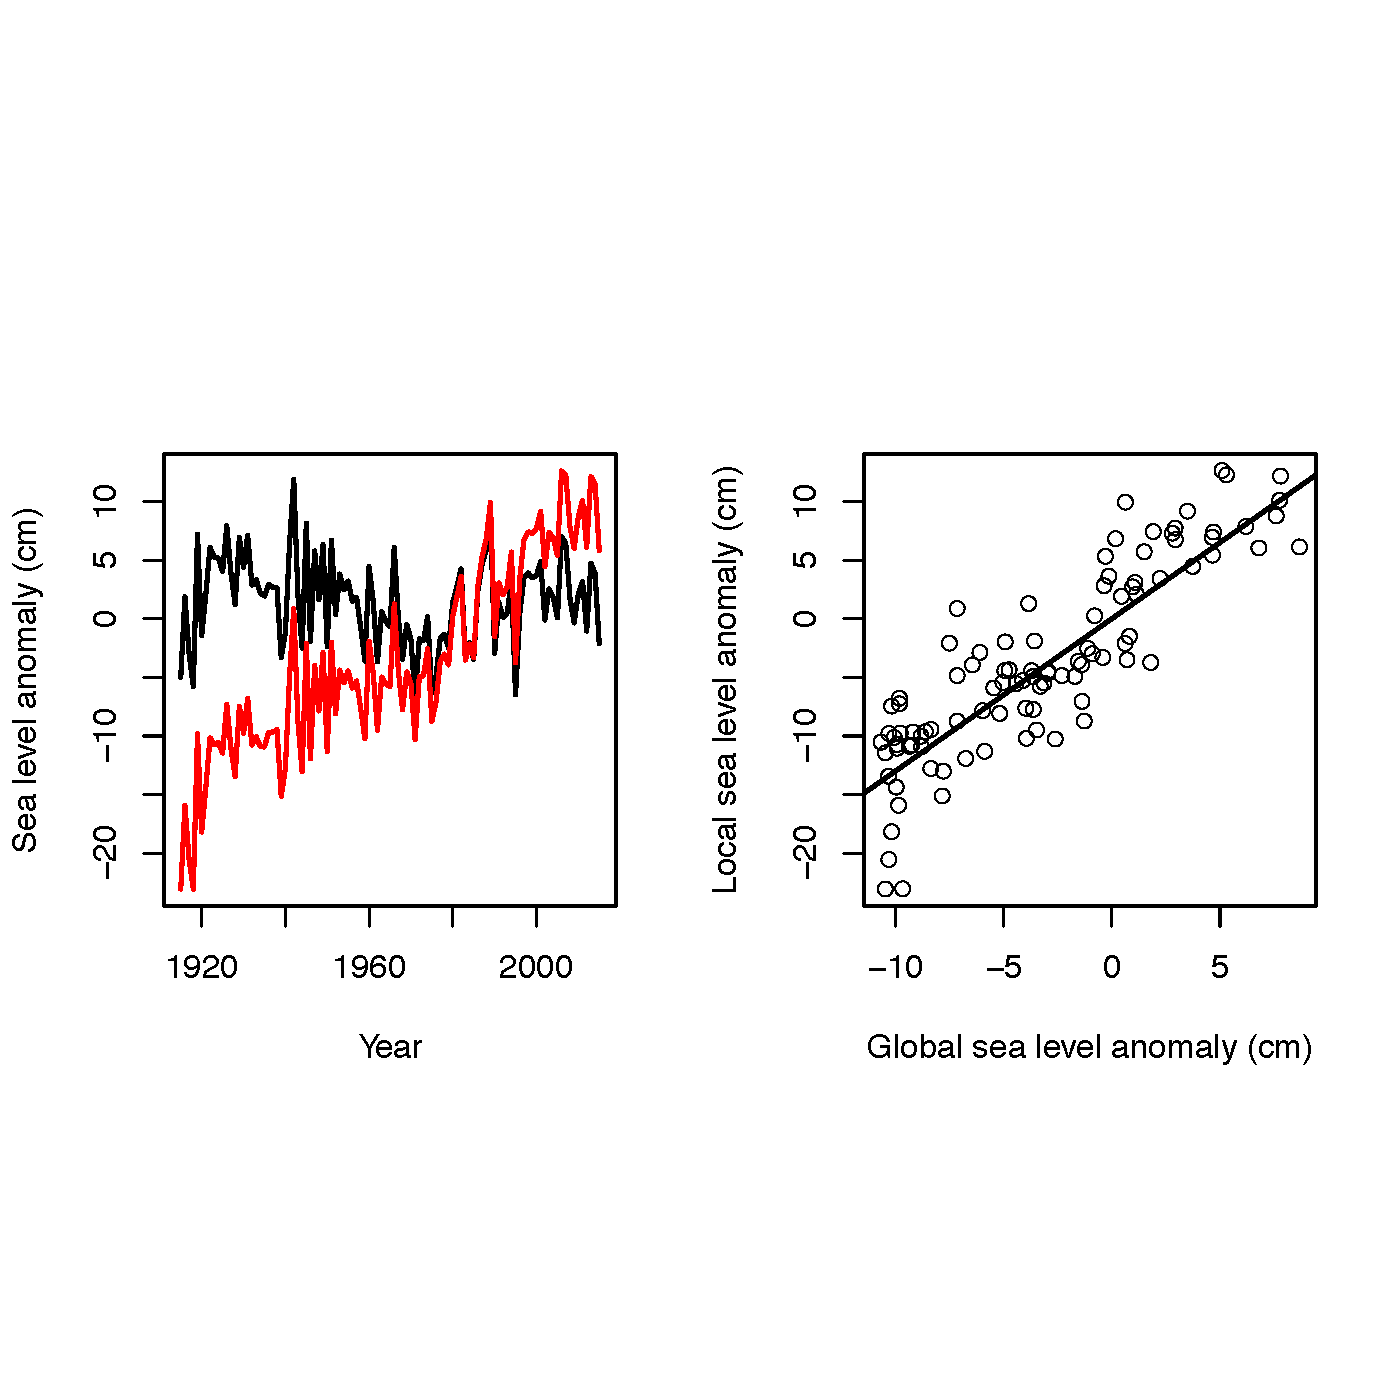
\includegraphics[width=\linewidth]{bergenfit.png}
\caption{ The left figure shows raw (black)and gia-corrected (red) sea level data from Bergen, The right figure relates the gia-corrected Bergen sea level to the global sea level series of \citet{csiro}. The straight line is the time series regression line.}
\label{fig:bergenobs}
\end{center}
\end{figure}

For the relationship between global annual mean temperature and global annual mean sea level rise we use the results from \citet{Bolin2014a}. The left panel of figure \ref{fig:ci} shows the simultaneous 90 \% confidence region for Bergen sea level rise relative to 1999 under scenario RCP 8.5, which is the scenario Norwegian authorities recommend for planning purposes.
\begin{figure}[!hbpt]
\begin{center}
\begin{minipage}{.5\textwidth}

 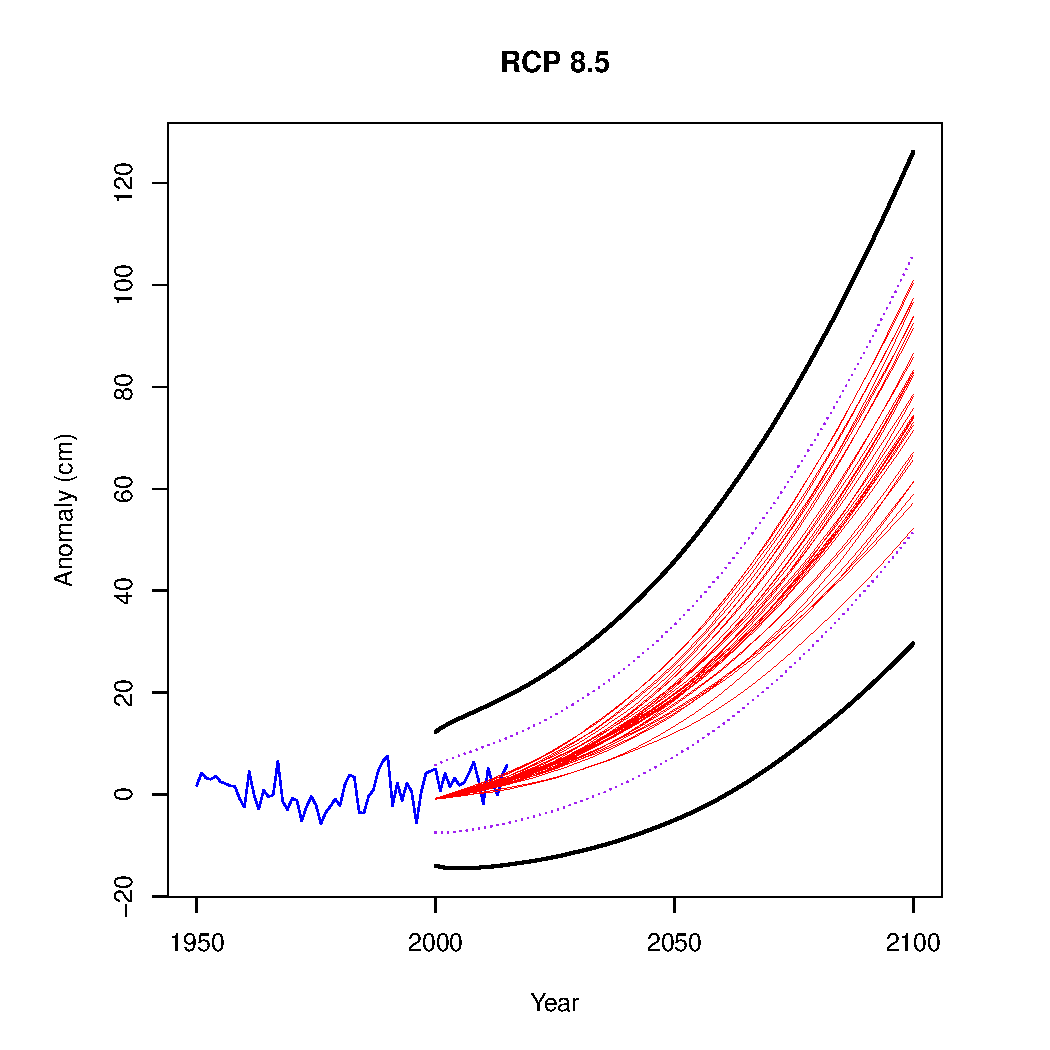
\includegraphics[width=\linewidth]{bergen_ci.pdf}
 % \label{fig:bergenci}

\end{minipage}%
\begin{minipage}{.5\textwidth}

    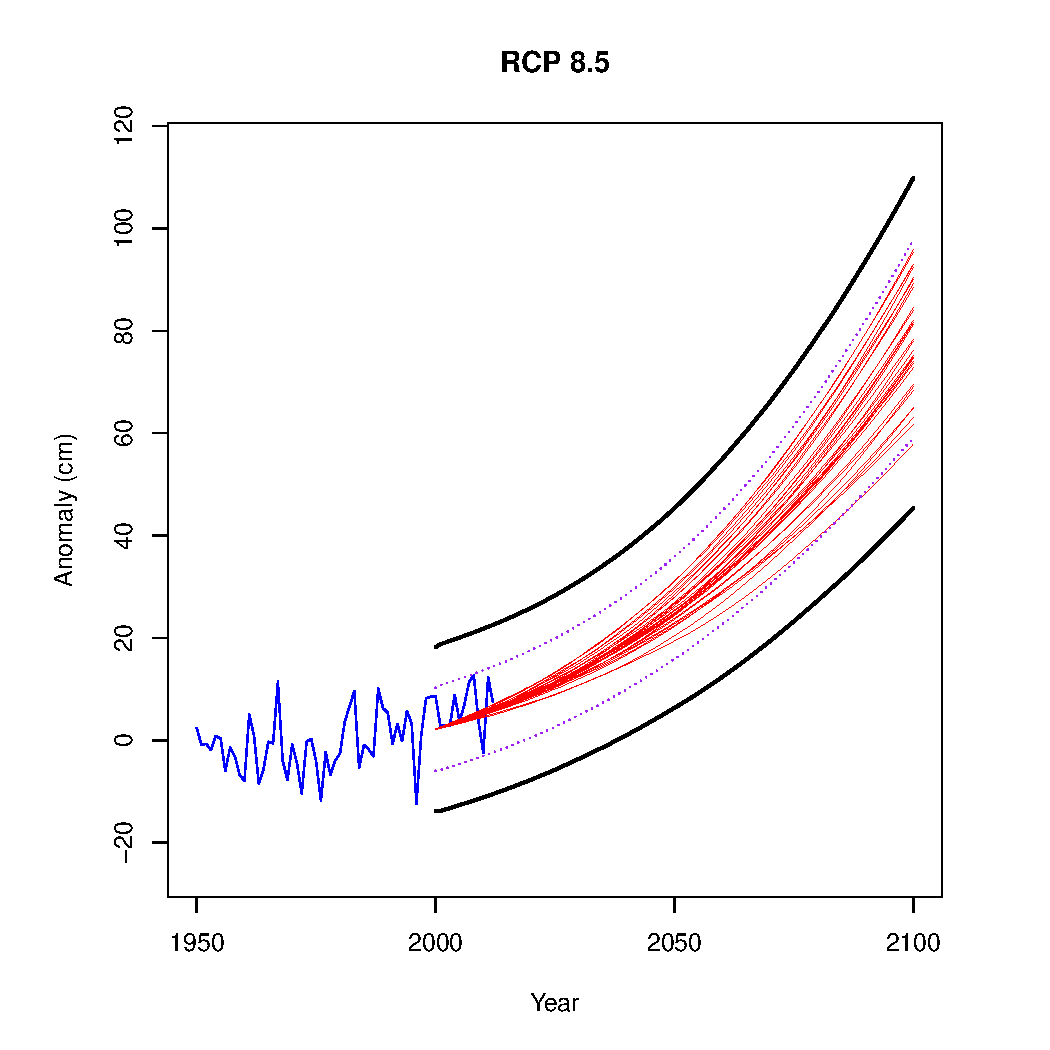
\includegraphics[width=\linewidth]{esbjerg_ci.pdf}
 % \label{fig:esbjergci}

\end{minipage}
\caption{Simultaneous 90\% confidence set (thick black lines) for Bergen (left) and Esbjerg( right) sea level projections for the years 2000-2100 using RCP8.5. The sea level data are shown in blue and end in 2015. The thin red lines are the projections without uncertainty based on each of the climate models. The dashed purple lines connect pointwise confidence intervals for each year. }
\label{fig:ci}
\end{center}
\end{figure}

For Esbjerg, the glacial isostatic adjustment is 0.06 (0.03) cm/yr. The time series regression model relating gia-corrected local to global sea level is an MA(1) model with parameter 0.17 (0.09). The regression slope is 1.02 (0.06). The right panel of figure \ref{fig:ci} shows the simultaneous 90\% confidence region for sea level rise relative to 1999 under scenario RCP 8.5.


\subsection{Timing of adaptation measures {\color{blue} (KdB, TT)}}

The histogram of the observed annual damages and the estimated distribution are given in Figure~\ref{fig:BergenDamageDist}. The parameter estimates for the Burr distribution are $\hat{\alpha} = 1.27$, $\hat{\gamma} = 0.51$ and $\hat{\theta} = 0.002$. 

\begin{figure}
\begin{center}
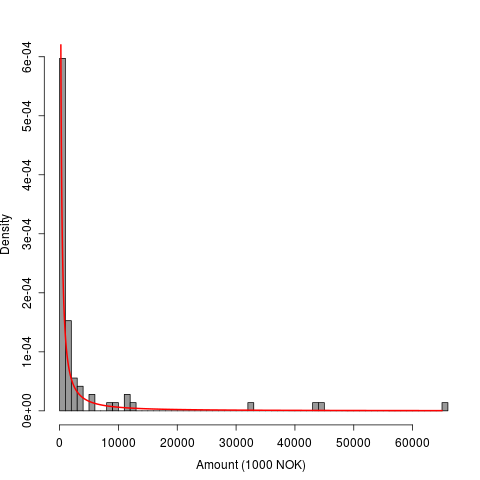
\includegraphics[width=\linewidth]{DamageDistribution.png}
\caption{ The estimated distribution of annual storm surge damage in Bergen for 2015 (red) based on observed annual damage in Hordaland and Rogaland 1980-2015 (gray bars). }
\label{fig:BergenDamageDist}
\end{center}
\end{figure}


For modelling the relationship between the change in damage and change in sea level we use the results of \cite{Hallegatte&2013} for 15 European cites: Amsterdam, Athens, Barcelona, Dublin, Glasgow, Hamburg, Helsinki, Copenhagen, Lisbon, London, Marseille, Naples, Porto, Rotterdam and Stockholm. \cite{Hallegatte&2013} estimate the mean annual flood damage in these cities in 2050 under no sea level change, 20 cm increase and 40 cm increase in sea level. We standardize their results for each city and consider the relative change for 20 and 40 cm increase. We then perform a linear extrapolation to obtain estimated relative changes in damage for a large interval of changes in sea level rise, see Figure~\ref{fig:ChangeInDamage}. Finally, the function $g$ is obtained by sampling from this ensemble of functions with all 15 ensemble members considered equally probable. 

\begin{figure}[!hbpt]
\begin{center}
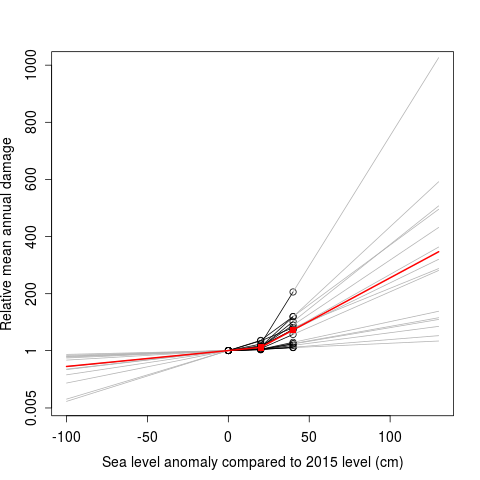
\includegraphics[width=\linewidth]{EuropeanIncreaseLossExtrapolationUncertainty.png}
\caption{ Relative change in mean annual damage as a function of sea level rise for 15 European cites as estimated by \cite{Hallegatte&2013} (black circles) with linearly extrapolated values indicated by gray lines. The median change and the corresponding extrapolation are indicated in red.}
\label{fig:ChangeInDamage}
\end{center}
\end{figure}


\begin{figure}[!hbpt]
\begin{center}
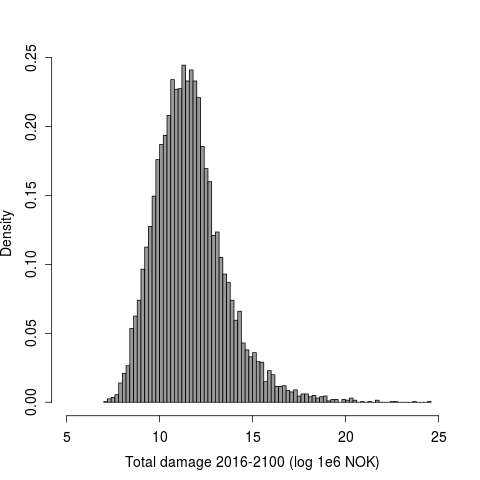
\includegraphics[width=\linewidth]{AccumulatedFutureLoss.png}
\caption{Distribution of log  accumulated future loss 2016-2100 under RCP 8.5 and assuming that no adaptation measures are implemented.} 
\label{fig:NoAction}
\end{center}
\end{figure}


\subsection{Selection of adaptation measures(?) {\color{blue} (MD)}}

A case study focusing on Denmark. 

\section{The value of including uncertainty}
\label{unc}

In many cases sea level rise projections are given as a single number for each scenario, usually the mean or median of the ensemble of projections from different climate models (e.g. \citet{climateimpactgroup}). Sometimes the spread of the ensemble is used to assess the uncertainty in the projections (e.g., the Norwegian Environmental Agency recommends using the upper ensemble value for RCP 8.5 as the basis for planning decision, pers. comm. from Even Nilsson, Norwegian Mapping Authority). In our analysiis there are two more sources of uncertainty, namely the two regression models. Figure \ref{fig:unc} shows the single number (vertical black line), the ensemble spread (histogram), the uncertainty including the global model (red) and the full uncertainty (blue) for Bergen projections of sea level rise relative to 1999 under RCP 8.5. We see that the ensemble range is about 16 cm, whereas the overall uncertainty range is about 40 cm.


\begin{figure}[!hbpt]
\begin{center}
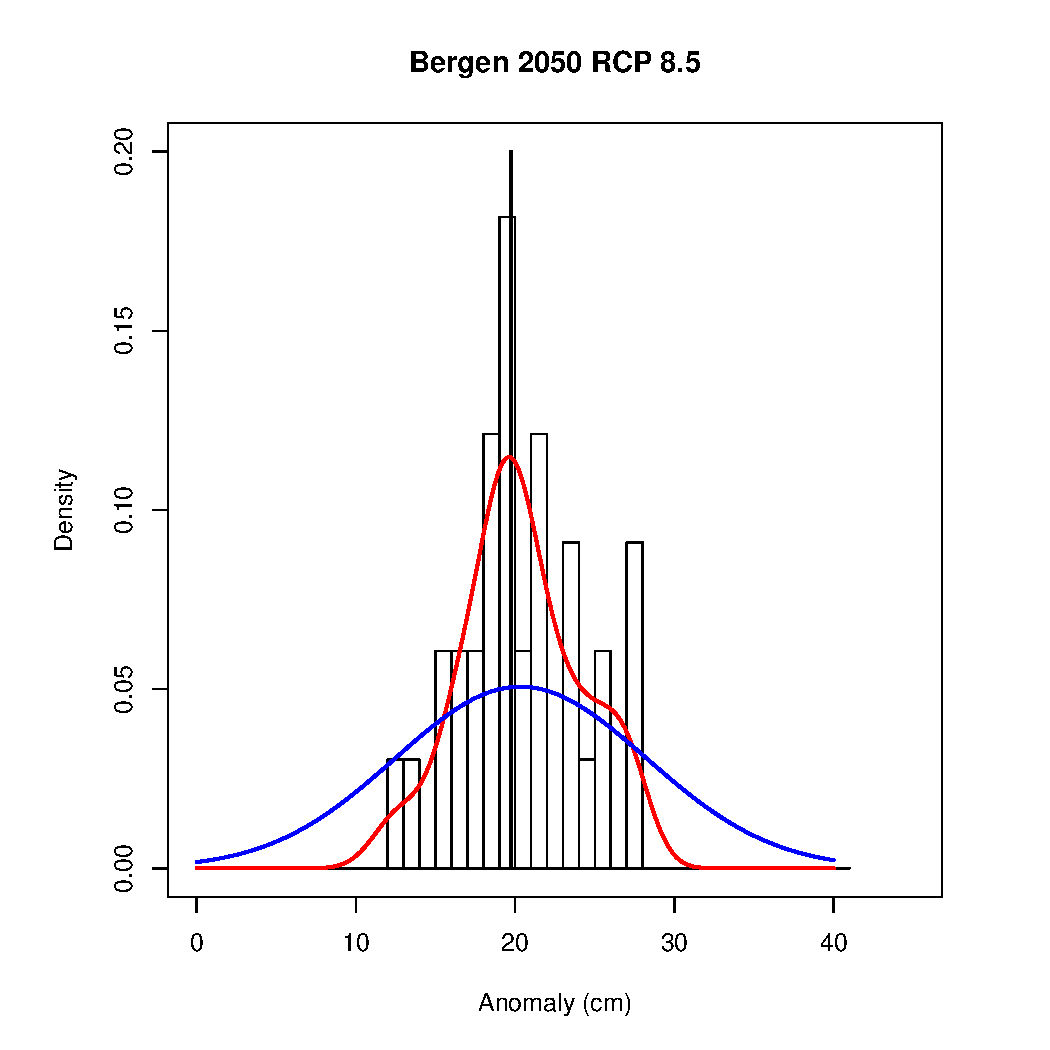
\includegraphics[width=\linewidth]{unc.pdf}
\caption{2050 Bergen sea level projections with uncertainty due to different sources for RCP 8.5. The black line is the median projection (with no uncertainty), while the grey histogram corresponds to the spread of the climate models, the red curve adds the uncertainty due to the relation between global temperature and global sea level, and the blue line that due to downscaling global sea level to Bergen. } 
\label{fig:unc}
\end{center}
\end{figure}





%  ACKNOWLEDGMENTS
\begin{acknowledgments}
This work was funded by NordForsk through project number 74456 ``Statistical Analysis of Climate Projections'' (eSACP) and The Research Council of Norway through project number 243953 ``Physical and Statistical Analysis of Climate Extremes in Large Datasets'' (ClimateXL). The source code for the analysis is implemented in the statistical programming language {\tt R} (\url{http://www.R-project.org}) and is available on GitHub at \url{http://github.com/eSACP/...}.
\end{acknowledgments}

%%  REFERENCE LIST AND TEXT CITATIONS
% 5\bibliographystyle{../BibTeX/agufull08}

\bibliography{ref.bib}
% Please use ONLY \citet and \citep for reference citations.

%\begin{thebibliography}{37}
%%   Before submitting: copy all the contents into the .bbl LaTeX file here
%%   and run latex again
%\providecommand{\natexlab}[1]{#1}
%\expandafter\ifx\csname urlstyle\endcsname\relax
%  \providecommand{\doi}[1]{doi:\discretionary{}{}{}#1}\else
%  \providecommand{\doi}{doi:\discretionary{}{}{}\begingroup
%  \urlstyle{rm}\Url}\fi


%\end{thebibliography}


%% Enter Figures and Tables here:

\end{document}
